\section{Introduction}


In recent years, the barriers to the development of Artificial Intelligence (AI) have been broken down with the rapid progress of ABC technologies in computing: AI, Big Data, and Cloud Computing, as well as the emergence of cost-effective specialized hardware~\cite{sze2017efficient} and software~\cite{jia2014caffe}. This has led to the world entering the third wave of AI development: Deep Learning~\cite{lecun2015deep}.
The success of current data-driven AI relies on massive amounts of training data and follows a gather-and-analyze paradigm~\cite{whang2023data}, which confronts with challenges of complying with rigorous data protection regulations such as OECD Privacy Guidelines~\cite{tene2011privacy} and General and Data Protection Regulation (GDPR)~\cite{voigt2017eu}.
So although data-centric AI is now the mainstream, a novel model-centric distributed collaborative training framework called Federated Learning is gaining popularity in both academia and industry due to its advantages in complying with privacy regulations.
So although data-centric AI is currently mainstream, Federated Learning (FL)~\cite{li2020federated}, a novel model-centric distributed collaborative training framework, is gaining popularity in both academia and industry for its advantages in complying with privacy regulations~\cite{truong2021privacy}.

According to the definitions of IEEE Standard for Federated Machine Learning (FML, aka FL)~\cite{IEEEstd3652}, \textit{FL is a framework or system that enables multiple participants to collaboratively build and use machine learning models without disclosing the raw and private data owned by the participants while achieving good performance.}
For example, a typical workflow of FL systems is that the entity with modeling demand (aka FL server) first deploys the FL services and initializes the model training task, and then distributing this task to participants with training data (aka FL clients) for modeling~\cite{bonawitz2019towards}.
Based on this workflow pattern, many FL frameworks have been derived with specialized improvements in communication~\cite{konevcny2016federated, mcmahan2017communication, xu2021asynchronous}, optimizaiton~\cite{li2018federated, karimireddy2020scaffold, li2021model}, robustness~\cite{duan2020self, sattler2019robust, li2022federated} and privacy~\cite{bonawitz2017practical, geyer2017differentially, cheng2021secureboost}.
While these fascinating improvements greatly enhance the utility of FL, they all follow a task-based interaction paradigm, in which an FL server dominates the cooperation between FL participants.
In this narrow interpretation of FL, the data owner is treated more like a worker than a collaborator and performs training primarily for the benefit of the server's goals.
Due to the above defects, clients have little enthusiasm to participate, and the potential for redundant training also leads to low model reuse rate, further diminishing the efficiency of the FL systems.
This explains why current FL frameworks are more akin to private distributed modeling services rather than sustainable and privacy-preserving modeling platforms for everyone as expected.

In this paper, we try to answer the question: \textbf{Can we establish a sustainable open FL platform based on a novel mutually beneficial cooperation framework?}
Obviously, to answer this quesion, it is insufficient simply study the basic concepts of FL and investigate existing FL techniques.
We also need to conduct a wide survey of potential techniques that can facilitate the construction of an open FL platform.
To aid understanding, Fig.~\ref{fig:coop} provides a first glimpse of two novel FL cooperation frameworks we advocated: 
\begin{itemize}
    \item \textbf{Query-based FL.} It follows a loosely-coupled cooperation framework between entities (we use "entities" instead of "participants" to emphasizes equality), where any entity can freely upload their local models or retrieve models from the open repository named Model Community.
    There are many valuable challenges that can be explored, such as how to query for models, how to "assemble" the retrieved models, or how to transfer knowledge from these models (see Section~\ref{}). %TODO: 
    \item \textbf{Contract-based FL.} It follows a mutual choice cooperation framework, where each entity can deploy model training contracts with specialized requirements such as task modality, execution environment, model architecture and license. Meanwhile, entities holding data can choose whether to accept the contract.
    Research topics in this area include model pricing, model ownership verification and .... (see Section~\ref{}) % TODO:
\end{itemize}
It's worth noting that the definitions of the four roles (i.e., model user, coordinator, data owner, auditor) are adopted for compatibility with the IEEE standard~\cite{IEEEstd3652}, and our proposals are also within the scope of FML definitions. 
The diagram in Fig.~\ref{fig:coop}(c) illustrates the workflow of traditional FL, where all FL clients are required to accept the training schedule from the FL server and perform multiple rounds of local training until the model converges.
In contrast, the entities in query-based FL and contract-based are proactive in their participate.
We believe that these mutually beneficial cooperation frameworks have the potential to expand the prevalence of FL and establish FL ecosystems.

\begin{figure}[b]
    \centering
    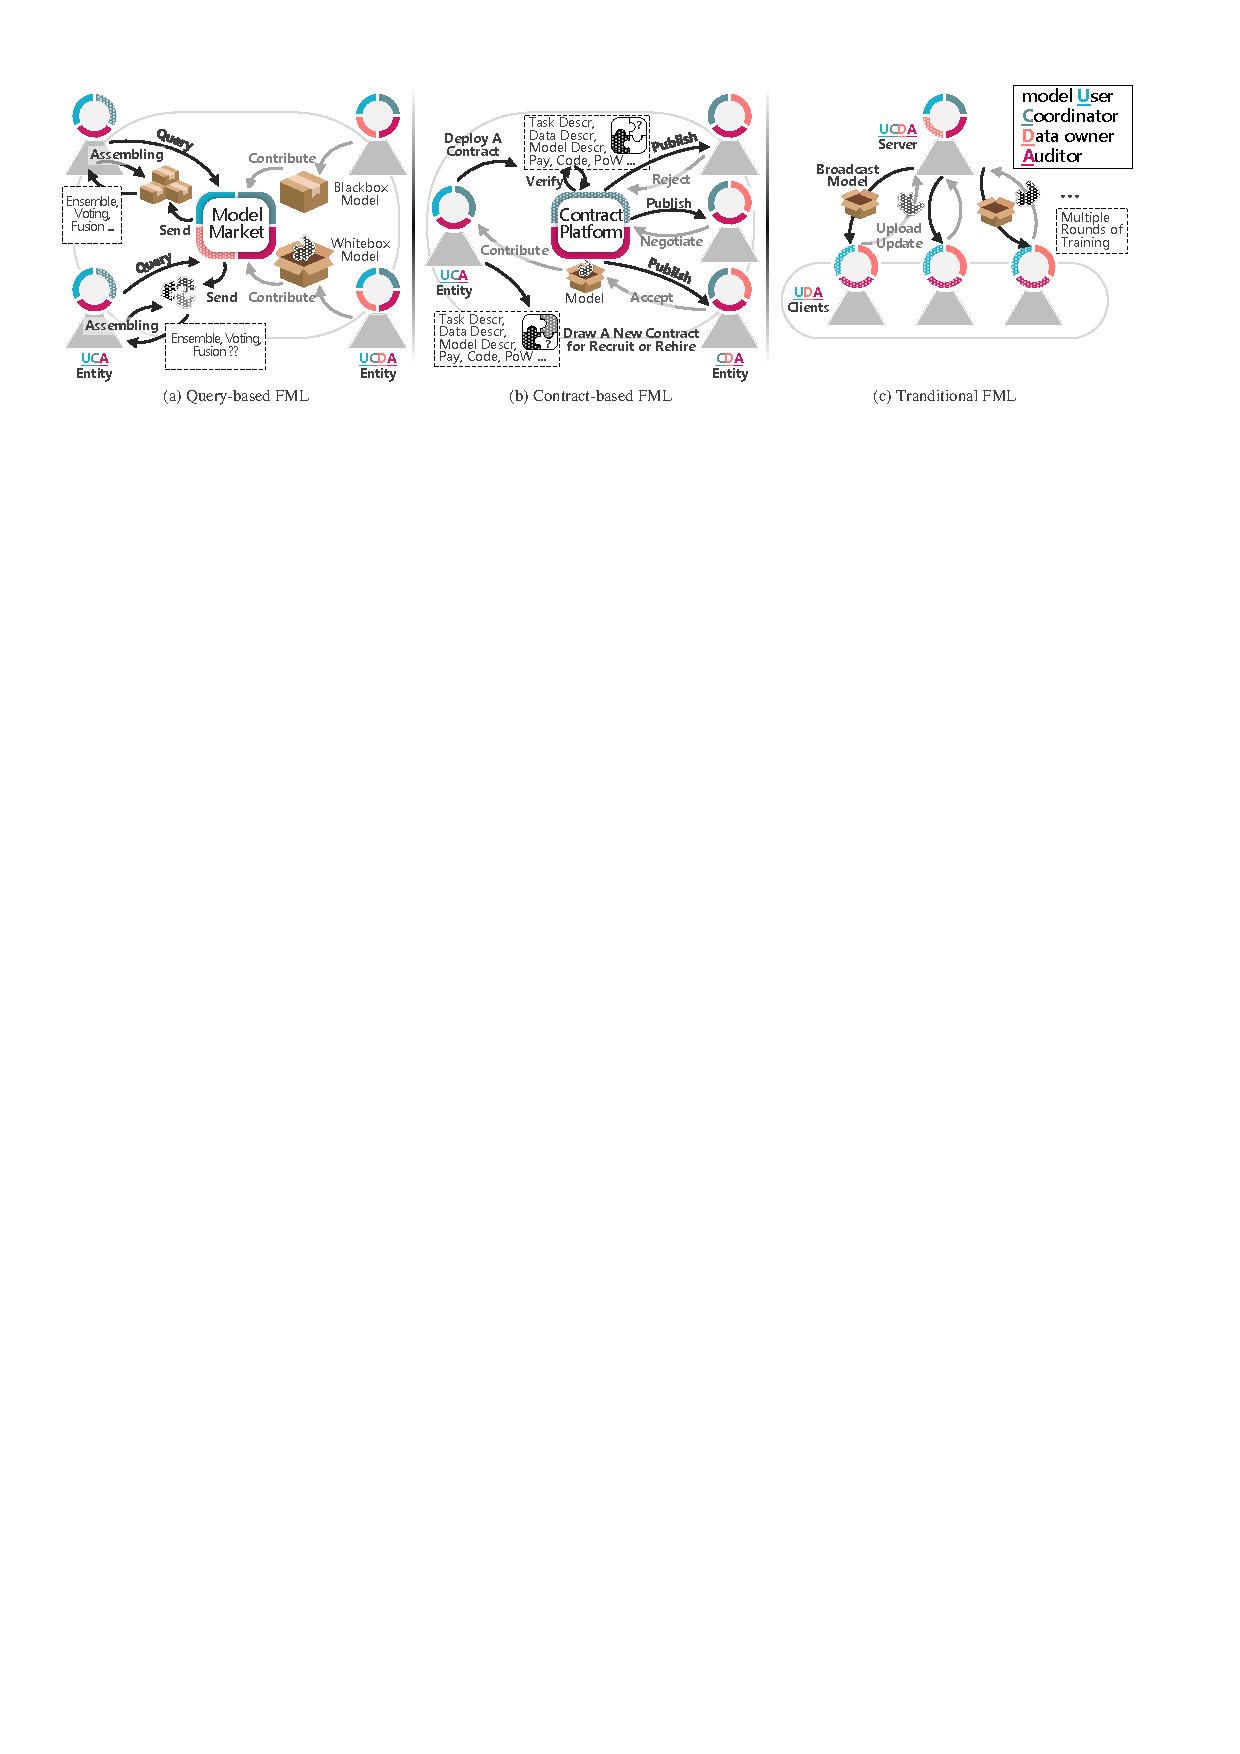
\includegraphics[width=\linewidth]{fig/coop_frame.pdf}
    \caption{A schematic diagram of three cooperation frameworks of FL. (a) (b) are the proposed open FL platforms, (c) is the traditional FL platform. Four colors correspond to four roles in~\cite{IEEEstd3652}, and colors with grid lines indicate non-essential roles.}
    \Description{}
    \label{fig:coop}
  \end{figure}

\subsection{Related Surveys}
Federated learning has become a buzzword in various fields, leading to the emergence of numerous FL studies.
These works can be classified into three primary categories: FL systems design, FL appllications and FL toolkits. Extensive surveys are available to summarized the advancement of federated learning, as shown in Table~\ref{table:surveys}.
The initial architectures and concepts for FL systems were summaried by Yang \textit{et al.}~\cite{yang2019federated}. 
They categorized FL into horizontal FL, vertical FL and federated transfer learning based on the distribution characteristics of data, 
which are written in IEEE Standard 3652.1-2020~\cite{yang2021white, IEEEstd3652}. 
Following this, an increasing number of surveys have emerged focusing on enhancing FL system design~\cite{li2020federated,aledhari2020federated, kairouz2021advances, zhang2021survey, li2021survey}. 
From the algorithmic perspective, personlized FL~\cite{kulkarni2020survey, tan2022towards} aims to learn personlized models for each client to address the challenge of statistical heterogeneity~\cite{ma2022state}.
Besides, the privacy-perserving computing platforms and model aggregation protocols for FL systems also been widely studied and sumaried by~\cite{liu2022privacy,el2022differential,yin2021comprehensive,lyu2020threats}.
Furthermore, many advanced FL architectures had been proposed, such as asynchronous~\cite{xu2021asynchronous}, decentralized and blockchain-based FL frameworks~\cite{nguyen2021federated, qu2022blockchain, zhu2022blockchain}.
Given that federated learning technologies enable collaboration among distributed participants in model training and decision-making, this capability holds great promise in a wide range of application scenarios.
For instance, multiple geogrphically distributed medical insitutions can enhace medication recommendation, drug-drug interaction prediction and medical image analysis in a collaborative manner without exchanging any sensitive data~\cite{xu2021federated, pfitzner2021federated, antunes2022federated, rieke2020future}. 
The massive real-time data generated by IoT devices in smart cities~\cite{zhang2022federated, ramu2022federated}, industries~\cite{boopalan2022fusion}, vehicles~\cite{du2020federated} has also sparked interest in exploring how FL technology can be used to deliver more advanced services such as intrusion detection, anomaly detection, fraud detection and network load prediction~\cite{agrawal2022federated, alazab2021federated, ghimire2022recent}.

As summarized in Table~\ref{table:surveys}, most surveys extensively discuss the challenges of efficiency, heterogeneity, privacy in FL systems design, with the surveys from blockchain fileds offering the most comprehensive review.
However, except for a few blockchain-based FL studies, most of the above surveys just present the same story from slightly different angles or backgrounds, i.e a server sets the model training task and delegate it to data holders to complete. 
This \textit{server-dominated} cooperation framework is a narrow implementation of the FL systems.
Therefore, this survey aim to fill the gap by investigating and surveying the associated tenchnologies that support more open and inclusive cooperation frameworks in FL systems, where all entities, whether they own the data or not, can benefit from it. 
The challenges investigated in this survey are not listed in the Table~\ref{table:surveys}, to the best of our knowledge, this is the first survey that focuses on the \textbf{cooperation frameworks} of FL.
In the following section, we will differentiate this survey from other related concepts in the field of FL.

\begin{table}[t]
    \footnotesize
    \caption{Summary of existing FL surveys, SYS denotes FL Systems Design, APP denotes FL Applications, SDC denotes Server-Dominated Cooperation frameworks.}
    \label{table:surveys}
    \begin{tabular}{|l|l|lllll|lll|}
    \hline
                       & \multicolumn{1}{c|}{} & \multicolumn{5}{c|}{Challenges}                                                                            & \multicolumn{3}{c|}{Contents}                            \\ \hline
                       Scenarios/Tasks &           FL Surveys            & \multicolumn{1}{l|}{Efficiency} & \multicolumn{1}{l|}{Heterogeneity} & \multicolumn{1}{l|}{Privacy} & \multicolumn{1}{l|}{Incentive} & Decentralized & \multicolumn{1}{l|}{SYS} & \multicolumn{1}{l|}{APP} & SDC \\ \hline
    \multirow{14}{*}{General} &      Yang \textit{et al.}~\cite{yang2019federated}         & \multicolumn{1}{c|}{ \checkmark } & \multicolumn{1}{c|}{\checkmark} & \multicolumn{1}{c|}{\checkmark} & \multicolumn{1}{c|}{\checkmark} & \multicolumn{1}{c|}{\checkmark}  & \multicolumn{1}{c|}{\checkmark} & \multicolumn{1}{c|}{\checkmark} & \multicolumn{1}{c|}{\checkmark}  \\ \cline{2-10}              
                        &   Li \textit{et al.} 2020~\cite{li2020federated}                    & \multicolumn{1}{c|}{\checkmark} & \multicolumn{1}{c|}{\checkmark} & \multicolumn{1}{c|}{\checkmark} & \multicolumn{1}{l|}{} & \multicolumn{1}{c|}{\checkmark} & \multicolumn{1}{c|}{\checkmark} & \multicolumn{1}{c|}{\checkmark} & \multicolumn{1}{c|}{\checkmark} \\ \cline{2-10} 
                        &   Zhang 2021\textit{et al.}~\cite{zhang2021survey}                    & \multicolumn{1}{c|}{\checkmark} & \multicolumn{1}{c|}{\checkmark} & \multicolumn{1}{c|}{\checkmark} & \multicolumn{1}{l|}{} &  & \multicolumn{1}{c|}{\checkmark} & \multicolumn{1}{c|}{\checkmark} & \multicolumn{1}{c|}{\checkmark} \\ \cline{2-10} 
                       &   Gupta \textit{et al.}~\cite{gupta2022survey}        & \multicolumn{1}{c|}{\checkmark} & \multicolumn{1}{c|}{\checkmark} & \multicolumn{1}{c|}{\checkmark} & \multicolumn{1}{l|}{} & \multicolumn{1}{c|}{\checkmark} & \multicolumn{1}{c|}{\checkmark} & \multicolumn{1}{c|}{\checkmark} & \multicolumn{1}{c|}{\checkmark} \\ \cline{2-10} 
                       &   Xu \textit{et al.}~\cite{xu2021asynchronous}                    & \multicolumn{1}{c|}{\checkmark} & \multicolumn{1}{c|}{\checkmark} & \multicolumn{1}{c|}{\checkmark} & \multicolumn{1}{l|}{} & \multicolumn{1}{c|}{\checkmark} & \multicolumn{1}{c|}{\checkmark} & \multicolumn{1}{c|}{\checkmark} & \multicolumn{1}{c|}{\checkmark} \\ \cline{2-10} 
                       &   Li \textit{et al.} 2021~\cite{li2021survey}        & \multicolumn{1}{c|}{\checkmark} & \multicolumn{1}{c|}{\checkmark} & \multicolumn{1}{c|}{\checkmark} & \multicolumn{1}{c|}{\checkmark} & \multicolumn{1}{c|}{\checkmark} & \multicolumn{1}{c|}{\checkmark} & \multicolumn{1}{c|}{\checkmark} & \multicolumn{1}{c|}{\checkmark} \\ \cline{2-10} 
                       &        El \textit{et al.}~\cite{el2022differential}               & \multicolumn{1}{l|}{} & \multicolumn{1}{l|}{} & \multicolumn{1}{c|}{\checkmark}& \multicolumn{1}{l|}{} & \multicolumn{1}{c|}{\checkmark} & \multicolumn{1}{c|}{\checkmark} & \multicolumn{1}{l|}{} & \multicolumn{1}{c|}{\checkmark} \\ \cline{2-10} 
                       &   Kulkarni \textit{et al.}~\cite{kulkarni2020survey}            & \multicolumn{1}{c|}{\checkmark} & \multicolumn{1}{c|}{\checkmark} & \multicolumn{1}{l|}{} & \multicolumn{1}{l|}{} &  & \multicolumn{1}{c|}{\checkmark} & \multicolumn{1}{l|}{} & \multicolumn{1}{c|}{\checkmark} \\ \cline{2-10} 
                       &  Liu \textit{et al.}\cite{liu2022privacy}             & \multicolumn{1}{c|}{\checkmark} & \multicolumn{1}{l|}{} & \multicolumn{1}{c|}{\checkmark} & \multicolumn{1}{l|}{} & \multicolumn{1}{c|}{\checkmark} & \multicolumn{1}{c|}{\checkmark} & \multicolumn{1}{l|}{} & \multicolumn{1}{c|}{\checkmark} \\ \cline{2-10} 
                       &    Tan \textit{et al.}~\cite{tan2022towards}     & \multicolumn{1}{l|}{} & \multicolumn{1}{c|}{\checkmark} & \multicolumn{1}{l|}{} & \multicolumn{1}{l|}{} &  & \multicolumn{1}{c|}{\checkmark} & \multicolumn{1}{l|}{} & \multicolumn{1}{c|}{\checkmark} \\ \cline{2-10} 
                       &           Zhu \textit{et al.} 2021~\cite{zhu2021federated}            & \multicolumn{1}{l|}{} & \multicolumn{1}{c|}{\checkmark} & \multicolumn{1}{l|}{} & \multicolumn{1}{l|}{} &  & \multicolumn{1}{c|}{\checkmark} & \multicolumn{1}{l|}{} & \multicolumn{1}{c|}{\checkmark} \\ \cline{2-10} 
                       &          Ma \textit{et al.}~\cite{ma2022state}            & \multicolumn{1}{c|}{\checkmark} & \multicolumn{1}{c|}{\checkmark} & \multicolumn{1}{c|}{\checkmark} & \multicolumn{1}{l|}{} &  & \multicolumn{1}{c|}{\checkmark} & \multicolumn{1}{l|}{} & \multicolumn{1}{c|}{\checkmark} \\ \cline{2-10} 
                       & Aledhari \textit{et al.}~\cite{aledhari2020federated}              & \multicolumn{1}{c|}{\checkmark} & \multicolumn{1}{c|}{\checkmark} & \multicolumn{1}{l|}{} & \multicolumn{1}{l|}{} &  & \multicolumn{1}{c|}{\checkmark} & \multicolumn{1}{c|}{\checkmark} & \multicolumn{1}{c|}{\checkmark} \\ \cline{2-10} 
                       &   Kairouz \textit{et al.}~\cite{kairouz2021advances}          & \multicolumn{1}{c|}{\checkmark} & \multicolumn{1}{c|}{\checkmark} & \multicolumn{1}{c|}{\checkmark} & \multicolumn{1}{c|}{\checkmark} & \multicolumn{1}{c|}{\checkmark} & \multicolumn{1}{c|}{\checkmark} & \multicolumn{1}{c|}{\checkmark} & \multicolumn{1}{c|}{\checkmark} \\ \cline{2-10} 
                       &      AbdulRahman \textit{et al.}~\cite{abdulrahman2020survey}   & \multicolumn{1}{c|}{\checkmark} & \multicolumn{1}{c|}{\checkmark} & \multicolumn{1}{c|}{\checkmark} & \multicolumn{1}{c|}{\checkmark} &  & \multicolumn{1}{c|}{\checkmark} & \multicolumn{1}{c|}{\checkmark} & \multicolumn{1}{c|}{\checkmark} \\ \cline{2-10} 
                       &    Lim \textit{et al.}~\cite{lim2020federated}       & \multicolumn{1}{c|}{\checkmark} & \multicolumn{1}{c|}{\checkmark} & \multicolumn{1}{c|}{\checkmark} & \multicolumn{1}{c|}{\checkmark} &  & \multicolumn{1}{c|}{\checkmark} & \multicolumn{1}{c|}{\checkmark} & \multicolumn{1}{c|}{\checkmark} \\ \hline
    \multirow{4}{*}{Healthcare}  &   Xu \textit{et al.}~\cite{xu2021federated}             & \multicolumn{1}{c|}{\checkmark} & \multicolumn{1}{c|}{\checkmark} & \multicolumn{1}{c|}{\checkmark} & \multicolumn{1}{l|}{} &  & \multicolumn{1}{c|}{\checkmark} & \multicolumn{1}{c|}{\checkmark} & \multicolumn{1}{c|}{\checkmark} \\ \cline{2-10} 
                       & Pfitzner \textit{et al.}\cite{pfitzner2021federated}                  & \multicolumn{1}{c|}{\checkmark} & \multicolumn{1}{c|}{\checkmark} & \multicolumn{1}{c|}{\checkmark} & \multicolumn{1}{l|}{} &  & \multicolumn{1}{c|}{\checkmark} & \multicolumn{1}{c|}{\checkmark} & \multicolumn{1}{c|}{\checkmark} \\ \cline{2-10} 
                       &           Antunes \textit{et al.}~\cite{antunes2022federated}             & \multicolumn{1}{l|}{} & \multicolumn{1}{c|}{\checkmark} & \multicolumn{1}{c|}{\checkmark} & \multicolumn{1}{l|}{} &  & \multicolumn{1}{l|}{} & \multicolumn{1}{c|}{\checkmark} & \multicolumn{1}{c|}{\checkmark} \\ \cline{2-10} 
                       &          Rieke \textit{et al.}~\cite{rieke2020future}             & \multicolumn{1}{l|}{} & \multicolumn{1}{c|}{\checkmark} & \multicolumn{1}{c|}{\checkmark} & \multicolumn{1}{l|}{} & \multicolumn{1}{c|}{\checkmark} & \multicolumn{1}{c|}{\checkmark} & \multicolumn{1}{c|}{\checkmark} & \multicolumn{1}{c|}{\checkmark} \\ \hline
    \multirow{4}{*}{IoT}  &   Zhang 2022\textit{et al.}~\cite{zhang2022federated}         & \multicolumn{1}{c|}{\checkmark} & \multicolumn{1}{c|}{\checkmark} & \multicolumn{1}{l|}{} & \multicolumn{1}{l|}{} &  & \multicolumn{1}{c|}{\checkmark} & \multicolumn{1}{c|}{\checkmark} & \multicolumn{1}{c|}{\checkmark} \\ \cline{2-10} 
                       &    Boopalan \textit{et al.}~\cite{boopalan2022fusion}    & \multicolumn{1}{c|}{ \checkmark } & \multicolumn{1}{c|}{\checkmark} & \multicolumn{1}{c|}{\checkmark} & \multicolumn{1}{c|}{\checkmark} & \multicolumn{1}{c|}{\checkmark}  & \multicolumn{1}{c|}{\checkmark} & \multicolumn{1}{c|}{\checkmark} & \multicolumn{1}{c|}{\checkmark}  \\ \cline{2-10}
                       &    Ramu \textit{et al.}~\cite{ramu2022federated}    & \multicolumn{1}{c|}{ \checkmark } & \multicolumn{1}{c|}{\checkmark} & \multicolumn{1}{c|}{\checkmark} & \multicolumn{1}{l|}{} & \multicolumn{1}{c|}{\checkmark}  & \multicolumn{1}{c|}{\checkmark} & \multicolumn{1}{c|}{\checkmark} & \multicolumn{1}{c|}{\checkmark}  \\ \cline{2-10}
                       &  Du \textit{et al.}~\cite{du2020federated} & \multicolumn{1}{c|}{\checkmark} & \multicolumn{1}{c|}{\checkmark} & \multicolumn{1}{c|}{\checkmark} & \multicolumn{1}{c|}{\checkmark} & \multicolumn{1}{c|}{\checkmark} & \multicolumn{1}{c|}{\checkmark} & \multicolumn{1}{c|}{\checkmark} & \multicolumn{1}{c|}{\checkmark} \\ \hline
    \multirow{3}{*}{Cybersecurity}  &  Agrawal \textit{et al.}~\cite{agrawal2022federated} & \multicolumn{1}{c|}{\checkmark} & \multicolumn{1}{c|}{\checkmark} & \multicolumn{1}{c|}{\checkmark} & \multicolumn{1}{l|}{} & \multicolumn{1}{c|}{\checkmark} & \multicolumn{1}{c|}{\checkmark} & \multicolumn{1}{c|}{\checkmark} & \multicolumn{1}{c|}{\checkmark} \\ \cline{2-10} 
                       &  Alazab \textit{et al.}~\cite{alazab2021federated}  & \multicolumn{1}{l|}{} & \multicolumn{1}{l|}{} & \multicolumn{1}{c|}{\checkmark} & \multicolumn{1}{l|}{} &  & \multicolumn{1}{c|}{\checkmark} & \multicolumn{1}{c|}{\checkmark} & \multicolumn{1}{c|}{\checkmark} \\ \cline{2-10} 
                       &  Ghimire \textit{et al.}~\cite{ghimire2022recent} & \multicolumn{1}{c|}{\checkmark} & \multicolumn{1}{l|}{} & \multicolumn{1}{c|}{\checkmark} & \multicolumn{1}{l|}{} &  & \multicolumn{1}{c|}{\checkmark} & \multicolumn{1}{c|}{\checkmark} & \multicolumn{1}{c|}{\checkmark} \\ \hline
    \multirow{3}{*}{Blockchain}  &  Nguyen \textit{et al.}~\cite{nguyen2021federated} & \multicolumn{1}{c|}{\checkmark} & \multicolumn{1}{c|}{\checkmark} & \multicolumn{1}{c|}{\checkmark} & \multicolumn{1}{c|}{\checkmark} & \multicolumn{1}{c|}{\checkmark} & \multicolumn{1}{c|}{\checkmark} & \multicolumn{1}{c|}{\checkmark} & \multicolumn{1}{c|}{\checkmark} \\ \cline{2-10} 
                       &  Qu \textit{et al.}~\cite{qu2022blockchain}  & \multicolumn{1}{c|}{\checkmark} & \multicolumn{1}{c|}{\checkmark} & \multicolumn{1}{c|}{\checkmark} & \multicolumn{1}{c|}{\checkmark} & \multicolumn{1}{c|}{\checkmark} & \multicolumn{1}{c|}{\checkmark} & \multicolumn{1}{c|}{\checkmark} & \multicolumn{1}{c|}{\checkmark} \\ \cline{2-10}
                       &  Zhu \textit{et al.} 2022~\cite{zhu2022blockchain} & \multicolumn{1}{c|}{\checkmark} & \multicolumn{1}{c|}{\checkmark} & \multicolumn{1}{c|}{\checkmark} & \multicolumn{1}{c|}{\checkmark} & \multicolumn{1}{c|}{\checkmark} & \multicolumn{1}{c|}{\checkmark} & \multicolumn{1}{c|}{\checkmark} & \multicolumn{1}{c|}{\checkmark} \\ \hline
                        &    & \multicolumn{1}{l|}{} & \multicolumn{1}{l|}{} & \multicolumn{1}{l|}{} & \multicolumn{1}{l|}{} &  & \multicolumn{1}{l|}{} & \multicolumn{1}{l|}{} &  \\ \hline
    \end{tabular}
    \end{table}

\subsection{Distinction of Our Survey}
This survey focuses on exploring the innovative cooperation frameworks in FL, which will involve some FL concepts such as decentralized FL, blockchain-based FL, few-shot FL, ML related platforms and services but goes beyond them.
In this section, we will distinguish our survey by highlingting the similarities and differences between these related concepts.

\subsubsection{Dcentralized FL}
ref:
given the high scalability of modern edge computing networks, a single MEC server cannot manage to aggregate all updates offloaded from millions of devices.
Therefore, there is an urgent need to develop a more decentralized FL approach without using a central server so as to solve security and scalability issues for enabling the next generation intelligent edge networks.

\subsubsection{Blockchain-based FL}

\subsubsection{Few-shot FL}

\subsubsection{FL Systems}
Federated learning, with its nature advantages in privacy-preserving decision sharing, has garnered significant attention in both industry and academia, leading to the rapid development of federated learning systems.
The earliest attempt at the large-scale FL system was by Google, where FL was used to improve next-word prediction~\cite{hard2018federated} and query suggesion~\cite{yang2018applied} for Gboard applications.
Subsequently, many novel FL systems have emerged to adapt to diverse federated training scenarios, such as Horizontal FL (e.g. TFF~\cite{abadi2016tensorflow}, FedLab~\cite{zeng2021fedlab}, Felicitas~\cite{zhang2022felicitas}, IBM FL~\cite{ibmfl2020ibm}), Vertical FL~\cite{wu2022practical} or both (e.g. FATE~\cite{liu2021fate}, FedML~\cite{he2020fedml}, PaddleFL~\cite{ma2019paddlepaddle}, Flower~\cite{beutel2020flower}, FedTree~\cite{li2022fedtree}, NVFLARE~\cite{roth2022nvidia}).
Despite these frameworks covering a wide range of application scenarios, they all follow the server-dominated cooperation mechanism.
This business model restricts FL to function as a collaborative modeling software, rather than an open platform that provides FL services to the public.

Unlike the FL systems mentioned above, PySyft~\cite{ziller2021pysyft} developed by OpenMined depicts a novel FL cooperation frameworks which is closely realted to our focus. 
PySyft encourages data owners to share their data on a private domain server, which provides data management and privacy controls, as well as limited machine learning analysis APIs for third-party data scientists.
Besides, a public network server will provide connections between data owners and data scientist, enabling datasets search and discovery for platform users.
Recently, a new FL platform named PySyTFF\footnote{https://blog.openmined.org/announcing-proof-of-concept-support-for-tff-in-pysyft-0-7/} was announced. It integrates TFF and PySyft, allowing data scientists to train models under the coordination of TFF and the datasets provided by PySyft domain servers.
However, even with inference controls of datasets, there is still a high security risk associated with exposing access to sensitive data on the Internet~\cite{gamundani2018review}.
To preserve the privacy advantages of FL, in this survey, we aim to discuss an open and data-free FL platform under the scope of model-centric ML~\cite{lou2020towards}.
In such FL platform, every user is free to collaborate on the training of machine learning models while privacy is protected.

\subsubsection{As-a-Service Business Model}

In the current context of Software-as-a-Service (SaaS)~\cite{brereton1999future}, there are several as-a-service cloud computing frameworks that encapsulate ML tasks as services and provides unified APIs for upper layer applications. 
For example, Model-as-a-Service (MaaS)~\cite{geller2007model, roman2009model, zou2012maas, liu2021jizhi, sun2022black} and Machine-Learning-as-a-Service (MLaaS)~\cite{ribeiro2015mlaas, hanzlik2021mlcapsule, hesamifard2018privacy,li2017scaling, kourtellis2020flaas} encapsulate model execution and model development as services.
The original concept of MaaS~\cite{geller2007model, roman2009model} was to provide re-usable and fine-grained user interfaces and visualization tools of domain-specific models (e.g wealther model, oil spill detection model) for environmental decision support systems.
Subsequently, this concept has been extended to the field of recommendation systems~\cite{zou2012maas} and deep learning based systems~\cite{liu2021jizhi, sun2022black}.
However, in contrast to the focus of this survey, the aforementioned MaaS framework does not involve any user collaboration but solely provides model inference APIs to users.

As the architectures of deep neural networks (DNNs) become increasingly complex, training and maintaining DNNs become more and more challenging~\cite{han2021pre}. To address this issue, cloud service providers have introduced MLaaS, which offers an integrated development environment as a service for constructing and operationalizing ML workflows, aiming to reduce the computational resources required.
MLaaS enables users to upload their data for training~\cite{ribeiro2015mlaas, zhao2021veriml, hesamifard2018privacy} or inference~\cite{hanzlik2021mlcapsule}, freeing them from the responsibility of managing hardware resources and implementation.
Most MLaaS providers adopt a pay-by-query business model, such as Google Vertex AI\footnote{https://cloud.google.com/vertex-ai}, Microsoft Azure Machine Learning\footnote{https://azure.microsoft.com/products/machine-learning/} and ChatGPT\footnote{https://chat.openai.com/chat}.
However, privacy protection can be compromised when users upload data to perform inference and training in the cloud.
Moverover, under this model, users are not given the ability to contribute their own models to the repository or collaborate with others to enhance the diversity of available models. 
While there are some ongoing efforts to offer privacy-preserving MLaaS services using techniques such as Isolated Execution Environment~\cite{hanzlik2021mlcapsule, mckeen2016intel} and Homomorphic Encryption~\cite{hesamifard2018privacy,gentry2009fully}, it is worth noting that our focus is not solely on privacy.
Rather, the FL framework we focus on emphasizes a collaborative framework where all entities involved have equal access to services and mutual benefits.

Recently, Kourtellis \textit{et al.}~\cite{kourtellis2020flaas} propose Federated Learning as a Service (FLaaS) that provides high-level and extensible APIs aim to enabling third-party applications to build collaborative, decentralized, privacy-preserving ML models.
However, this approach also follows the traditional server-dominated cooperation framework, which falls under the scope of previous FL surveys\cite{yang2019federated, li2020federated,kairouz2021advances}.

\begin{table}[t]
    \caption{Summary of existing deep learning model repositories.}
    \label{table:repository}
    \footnotesize
    \begin{tabular}{|l|c|c|c|c|c|c|c|c|}
    \hline
    & \multicolumn{1}{l|}{DS Name} & \multicolumn{1}{l|}{Model Architecture} & \multicolumn{1}{l|}{Modality/Task} & \multicolumn{1}{l|}{Tag} & \multicolumn{1}{l|}{License} & \multicolumn{1}{l|}{Input-Output} & \multicolumn{1}{l|}{Batch Export} & \multicolumn{1}{l|}{\# of Models}\\ \hline
    Hugging Face\tablefootnote{https://huggingface.co}
    & \checkmark & \checkmark & \checkmark & \checkmark & \checkmark & \textbf{!} & \ding{55} & 133,641 \\ \hline
    Model Zoo\tablefootnote{https://modelzoo.co/} & \checkmark & \checkmark & \checkmark & \checkmark & \ding{55} & \ding{55} & \ding{55} & 3,426 \\ \hline
    OpenVINO\tablefootnote{https://docs.openvino.ai/latest/model\_zoo.html} & \textbf{!} & \checkmark & \checkmark & \ding{55} & \textbf{!} & \textbf{!} & \checkmark & 278 \\ \hline
    Tensorflow Hub\tablefootnote{https://tfhub.dev/}& \checkmark & \checkmark & \checkmark & \checkmark & \textbf{!} & \textbf{!} & \ding{55} & 1,356 \\ \hline
    Pytorch Hub\tablefootnote{https://pytorch.org/hub/} & \textbf{!} & \checkmark & \ding{55} & \ding{55} & \ding{55} & \textbf{!} & \ding{55} & 49 \\ \hline
    NVIDIA NGC\tablefootnote{https://catalog.ngc.nvidia.com/models} & \textbf{!} & \checkmark & \checkmark & \checkmark & \textbf{!} & \textbf{!} & \ding{55} & 527 \\ \hline
    \end{tabular}
\end{table}

\subsection{FAIR in FL}
FAIR Data Principles: Findable, Accessible, Interoperable, Reusable.


\begin{comment}
    ssssdd

\end{comment}